\section{Interfejs użytkownika}
    
    \subsection{Górna belka}
        W górnej części aplikacji znajduje się menu kontekstowe. Pozwala ono na wywołanie okna inicjalizującego połączenie z serwerem (patrz \ref{fig:app_connect}). Do nawiązania pomyślnego połączenia wymagane jest umieszczenie poprawnego adresu oraz portu brokera MQTT. W przypadku dezaktywowanej opcji przyjmowania anonimowych użytkowników wymagane jest także podanie ważnych danych autoryzacyjnych.
        
        \begin{figure}[ht]
            \centering
            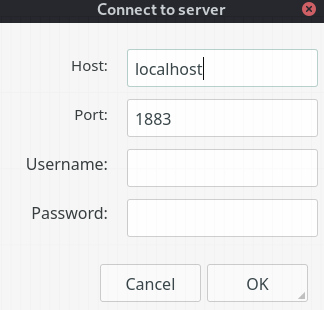
\includegraphics[width=0.5\textwidth]{img/app_connect.png}
            \caption{Okno nawiązywania połączenia}
            \label{fig:app_connect}
        \end{figure}
    
    
    \subsection{Panel parametrów}
        Dolna część okna podzielona jest na trzy części.
        
        \begin{itemize}
            \item Panel parametrów regulatora.
            \item Panel widoczności wykresów.
            \item Panel z aktualnymi danymi.
        \end{itemize}
        
        Pierwsza z nich udostępnia interfejs do dynamicznej zmiany nastaw regulatora 

    \subsection{Graf}
    Interfejs zawiera wszystkie elementy niezbędne do wygodnej obsługi urządzenia.
    
    \begin{figure}[ht]
        \centering
        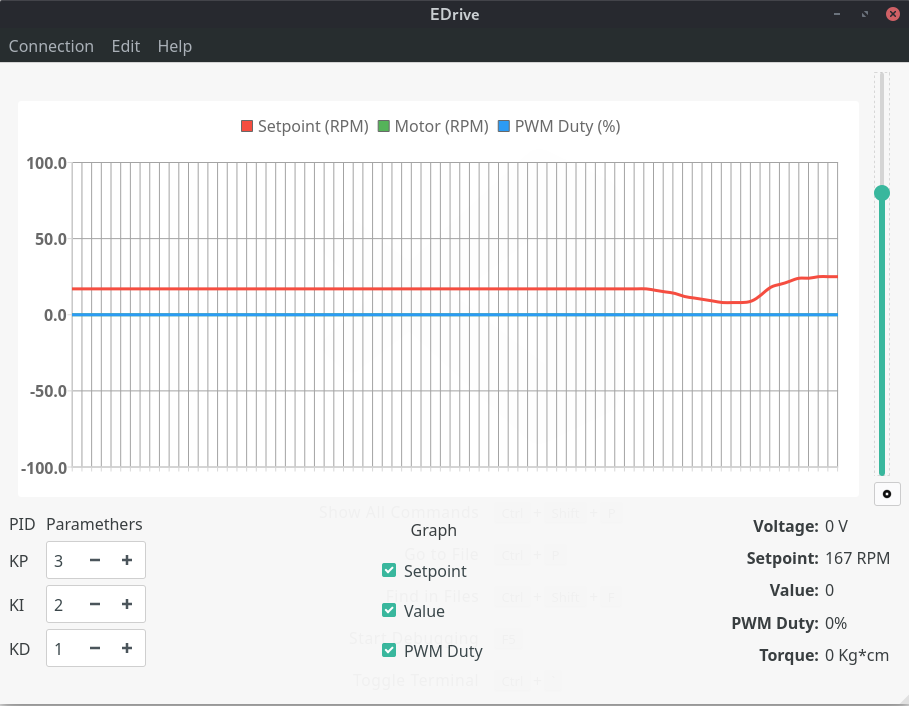
\includegraphics[width=1\textwidth]{img/app_ui.png}
        \caption{Interfejs użytkownika}
        \label{fig:app_ui}
    \end{figure}